In order to have data on which to perform analysis, we had to gather a large number of tweets from Twitter using the Twitter Search API. 

\subsection{Design Considerations}

While designing and implementing the tweet harvester, there were several major design considerations taken into account.

\subsubsection{Geographical limitation}

As the purpose of this assignment is to perform analysis on tweets from Australian cities, the tweet harvester must be able to gather the tweet data from specific locations only. Tweet objects from the Twitter API offer three location-related fields: \texttt{location}, \texttt{geo}, and \texttt{place}. Of these, \texttt{geo} is deprecated, so its value was ignored.

The fields \texttt{location} and \texttt{place} offer location data for a tweet in very different formats, and have different meanings. \texttt{location} is a GeoJSON \texttt{Point} feature indicating the $(longitude, latitude)$ location from which the tweet was sent. \texttt{place} is a more general positional identifier for a tweet, given as a Twitter Place. As a tweet with a Twitter Place is not guaranteed to be sent from the place and could just be about it, \texttt{coordinates} was chosen as the primary determiner of tweet location. In order to facilitate gathering tweets only from specific locations, tweet location must be filtered against some pre-determined location bounds, while tweets without a populated \texttt{coordinates} field are discarded entirely.

\subsubsection{Deduplication of tweets}

As indicated in the brief, a key aspect of the system design was ensuring that duplicate tweets do not and cannot occur in the corpus of gathered data. Twitter provides a unique identifier for tweets and users, which allows uniqueness in the CouchDB database to be enforced simply by using the tweet identifier as the document key.

\subsubsection{Twitter API status endpoints}

There are three key Twitter API endpoints available for gathering statuses:
\begin{enumerate}
    \item Search API: searching for a large number of tweets from the previous 7 days\footnote{For the Standard Search API. The Premium and Enterprise Search APIs allow access to either tweets from the previous 30 days or the full historical tweet archive.}.
    \item Real-time stream API: a real-time stream of tweets as they are posted.
    \item User timelines: access to up to 3,200 tweets from a user's timeline.
\end{enumerate}

To effectively gather large numbers of tweets, the harvester should use all three of them in combination.

\subsubsection{Search space expansion}

The combination of the Search and real-time stream APIs provides a good initial point from which to gather tweet data; however, the Search API has a limit of 7 days of tweets, while the real-time stream API is limited to the rate at which tweets are made in the location bounds. There are two obvious pieces of accessible information which are promising candidates for supplementing the other APIs: a user's followers, and a user's "friends"---the users they follow.

\subsubsection{Information redundancy}

A tweet contains a large amount of information, including many fields which are deprecated. Only the fields which contain relevant information are worth storing, as there is a finite amount of available disk space in which to store tweets. Because of this, tweets should be trimmed down to only the relevant fields before being stored in the CouchDB database.

\subsubsection{Rate limits}

Twitter's API enforces rate limits in order to prevent overwhelming numbers of requests being made, typically in the form of a maximum number of requests per 15 minute period. This inherently limits the maximum efficiency of the harvester, as it will spend the majority of its time waiting for rate limits to expire. This means it should be designed such that the impact of rate limits are minimised.

\subsection{Initial Design}

\begin{figure}[H]
    \centering
    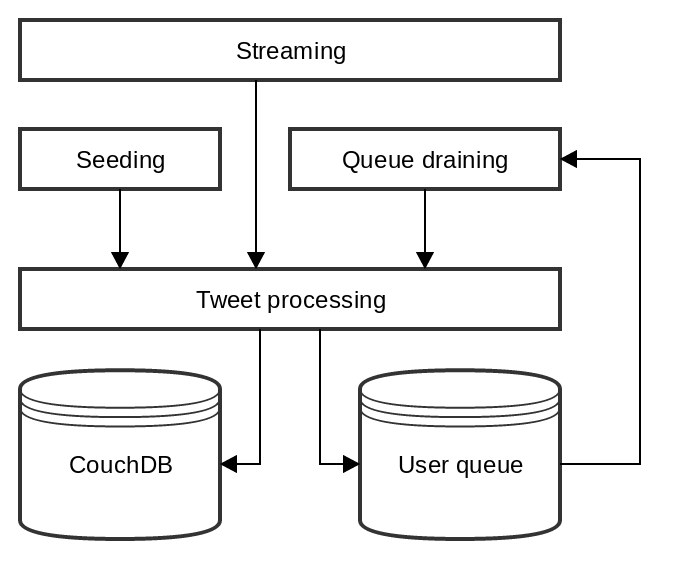
\includegraphics[width=8cm,keepaspectratio=true]{images/harvester.png}
    \caption{Tweet harvester design}
    \label{fig:harvesterinitdesign}
\end{figure}

\subsubsection{Configuration}

Harvester configuration is provided in the form of a \texttt{config.ini} file parseable by the Python standard library module \texttt{configparser}.

\subsubsection{User queue}

The harvester's design is based around a FIFO user queue. The user queue is the pool of users whose timelines to explore, and is drained and constantly refilled while the harvester is running.

\paragraph{Seeding}
Initially empty, the queue is populated through a seeding process where tweets are collected via the Search API and the users who post tweets with locations are added to the queue. In the initial harvester, the number of tweets to use as the seed was limited to a fixed value of 2000.

\paragraph{Queue draining}
Once seeding has completed, the harvester begins the process the contents of the user queue. It dequeues the first user, downloads a page of their timeline (up to 200 tweets), and processes each tweet. If no tweets which fall in the relevant location are found in the first page, the processing of the user is finished and the harvester will begin processing the next user. If tweets with desired locations \textit{are} found, it then proceeds to download and process all of the user's remaining tweets, and then queues the user's followers to be processed.

The decision to expand the search space using a user's followers rather than their friends was made based on an assumption of spatial proximity: an average Twitter user is likely to be followed by people they know or who have a low number of degrees of separation from them, while their friends are more likely to converge on a small pool of users with very large numbers of followers. If this assumption holds true, queuing followers is less likely to diverge spatially from the desired location, resulting in less wasted effort and more useful processing done between rate limits.

\subsubsection{Tweet processing}

Tweets are processed by the harvester in two ways: determining whether they have a location of interest, and whether their text is relevant to the story. If tweets have a location of interest, they are stored in the bulk CouchDB database and the user who posted the tweet is queued for further processing. If the tweet is also relevant to the story, it is additionally stored in a separate database containing only story-relevant tweets.

If a tweet is determined to be relevant in either way, the user who posted it is added to the user queue.

\subsubsection{Storing tweets}

Tweets are stored in the database using their ID as provided by Twitter as the document key. This allows the harvester to only store each tweet once, as it can check if the tweet already exists by checking if a document with the same key already exists. If such a tweet already exists, the harvester does not attempt to store it again, nor to update the existing document.

When tweets are stored in the database, they are pared down to a subset of the fields provided by the Twitter API, discarding deprecated and irrelevant fields.

\subsubsection{History}

In order to reduce wasted effort, the harvester stores a history of both processed users and tweets.

Tweets which have been processed already are ignored, which primarily occurs for the tweets which cause a user to be added to the queue---the tweet is processed before the user is added, then when the user is dequeued and processed the tweet will be found in their timeline again.

User history is used to determine whether or not to add the user to the queue---when a user is queued they are added to the history and will not be queued again. This means users who are found in more than one way, such as both by seeding and streaming, are not added to the queue multiple times.

\subsubsection{Streaming}

The harvester constantly monitors the real-time stream of tweets via the streaming API, essentially acting as a continuous seeding process.

\subsubsection{Multiple instances}

In order to harvest more tweets and to reduce the impact of rate limits, multiple harvesters are run simultaneously, each with its own credentials. As the processing history is instance-specific, the harvesters in the initial design operated on different subsets of Melbourne in order to avoid processing overlap. This has the limitation of a user possibly posting tweets in multiple areas governed by different harvesters, resulting in their reprocessing, but this was considered a relatively small cost.

\subsection{Challenges and refinements}

While the initial harvester implementation was moderately effective at gathering tweets, it had some drawbacks unaccounted for by the original design.

\subsubsection{User priority}

In the initial harvester design, users were removed from the queue in the same order they were added. This means there was no distinction between users who are known to post tweets with locations, such as those gathered from seeding or the real-time stream, and those who are not known to do so. Combined with the unbounded queue expansion from adding followers, this led to users known to post useful data to possibly never be processed.

In order to address this, the user queue was modified to be a priority queue, where priority of a user was determined by the way in which they were found: highest priority was given to users found via the real-time stream, while lowest priority was given to otherwise unknown followers. This improved the harvester efficiency and yield by guaranteeing that users who are known to post useful data are processed first.

\subsubsection{Users with many followers}

The initial harvester design queued \textit{all} followers of a user who posted relevant tweets. This functions well for an average user, but occasionally the harvester will encounter a user with a very large number of followers. Queuing all of the followers for one of these users will cause the harvester to hit the rate limits many times just for their followers. As an example, it took several hours to process all 896,000 followers of the user \textit{@ARTEM\_KLYUSHIN}\footnote{\url{https://twitter.com/ARTEM_KLYUSHIN}}.

In order to mitigate this, a limit on the number of followers to queue for any user was introduced, queuing only 400 followers at most. This provided enough new users in the queue to account for the low chance of any given user posting relevant tweets while also preventing users with many followers from taking a significant amount of time to process.

\subsubsection{Processing restart on redeployment}

The processing history was not persistent, which is acceptable for long-running sessions, but can cause the harvester to reprocess users after the restart or redeploy. As tweets are not added to the database if they are already known, this effort is entirely wasted and causes rate limits to be hit without yielding useful data. This problem was exacerbated by the incremental nature of development; as new features were introduced or bugs fixed, the harvester would continually be reset, causing reprocessing to occur multiple times.

This problem was mitigated by the introduction of a processed user database. This database contains documents indicating users who have already been processed or are currently being processed by a harvester instance, keyed by user ID. Before processing a user, a harvester checks if the user already exists in the processed users database, and if they do then the user is not processed. This allows the user history to persist over harvester restarts, reducing the amount of reprocessing done.

A side effect of this change was to allow harvesters to operate on the same region, due to giving access to a shared user history. A user is added to the user database at the beginning of an instance processing that user, other harvesters which have the user queued won't further process it. If a user has already been processed, the harvester has a random 25\% chance to queue their followers. This randomisation serves two purposes: firstly, it means that when a harvester is restarted and only finds processed users during seeding, it will still have a pool of users to process further; and secondly, it forces multiple harvester instances out of sync with each other, which means it is unlikely that multiple harvesters will be checking whether a user exists in the database at once, reducing the chances of a data race.

\subsubsection{Seed search term}

As the Search API requires a search query, a seed search term was used, the initial value of which was ``Melbourne'', chosen as it would likely yield tweets about locations within the area of interest, and because it was generic enough that it would be useful while we determined the story we would investigate.

Once the story was decided the search term was modified to be terms related to our topic of interest, increasing the likelihood of the seed tweets being useful. Due to the topic of interest being narrower than ``Melbourne'' as a search term, the fixed cap on seed size was removed, allowing all returned tweets from the past 7 days to be used as a seed.

\subsubsection{Error handling}

As the twitter harvester was implemented using \texttt{Tweepy}\footnote{\url{https://www.tweepy.org/}}, handling for errors such as hitting rate limits came at little to no cost. However, for errors not handled by \texttt{Tweepy}, additional error handling was required.

The primary error encountered by the tweet harvester was sporadic 401 - Not Authorized responses from the Twitter API while traversing a user's timeline. Twitter offers very little information from which to debug the cause of authorisation errors, which, combined with the intermittent and inconsistent nature of the errors, made robust error handling difficult. Instead, a best-effort approach was taken, where an authorisation error would merely cause the harvester to finish processing the current user and log the error, before moving onto the next queued user.

As the harvester requires databases exist in CouchDB before it can gather tweets, it creates them automatically when it is initialised, allowing the harvester to begin gathering tweets immediately.


